\subsection{Módulo Administrador de centro}

  \paragraph{}El diagrama de la figura
  \ref{diagramaDescomposicionAdministradorCentro} representa el módulo
  Administrador de centro. En primer lugar, el usuario administrador de centro
  debe validar sus datos de acceso para que se permita o no el acceso a las
  funciones de las que se compone el módulo.

  \paragraph{}Desde este módulo, el administrador de centro podrá acceder a
  todos los procesos necesarios para organizar correctamente toda la estructura
  de información de la que se compone el centro al que pertenece.

  \paragraph{}Además cuenta con un módulo de ayuda disponible en todo momento
  para el correcto manejo de la aplicación.

  \begin{figure}[!ht]
    \begin{center}
      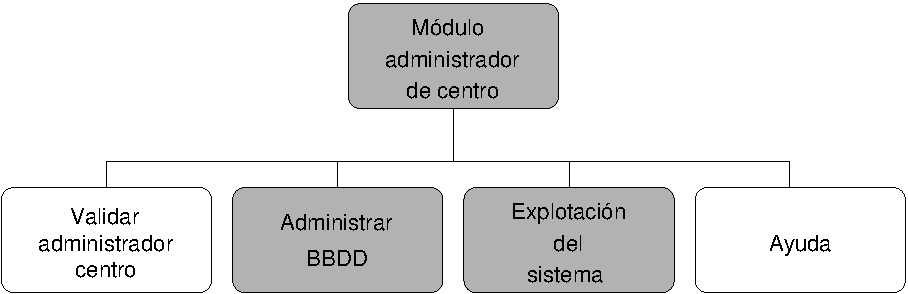
\includegraphics[]{11.Disenyo_Arquitectonico/11.2.Diagramas_Descomposicion/11.2.3.Modulo_administrador_centro/Diagramas/administrador_centro.pdf}
      \caption{Diagrama de descomposición del módulo Administrador de centro.}
      \label{diagramaDescomposicionAdministradorCentro}
    \end{center}
  \end{figure}

\paragraph{}El usuario administrador principal puede gestionar centros,
departamentos, titulaciones, asignaturas, asesores, alumnos y plantilas
oficiales de la base de datos.

\paragraph{}La figura \ref{diagramaNivel3-AdministrarBBDD-adminPrincipal}
muestra el nivel de abstracción 3: Administrar BBDD (módulo Administrador
principal).

  \begin{figure}[!ht]
    \begin{center}
      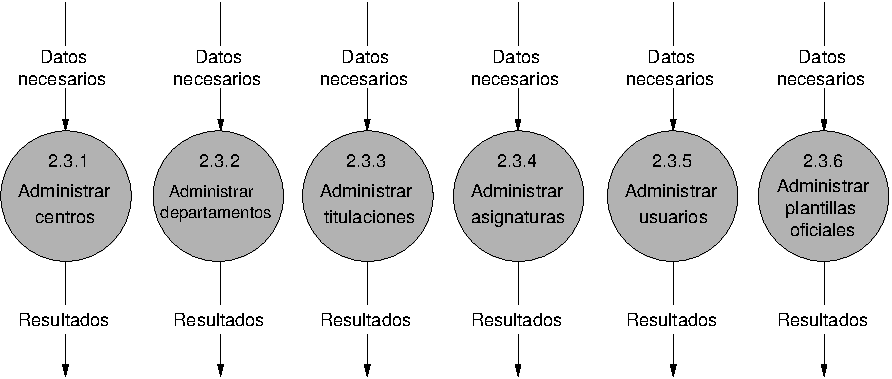
\includegraphics[]{08.Analisis_Funcional/8.2.DFDs/Niveles/Nivel3/AdministradorPrincipal/AdministrarBBDD/Diagramas/nivel3-AdministrarBBDD.pdf}
      \caption{Nivel de abstracción 3: Administrar BBDD (módulo Administrador
      principal).}
      \label{diagramaNivel3-AdministrarBBDD-adminPrincipal}
    \end{center}
  \end{figure}
